%% Template for MLP Coursework 1 / 16 October 2017

%% Based on  LaTeX template for ICML 2017 - example_paper.tex at
%%  https://2017.icml.cc/Conferences/2017/StyleAuthorInstructions

\documentclass{article}

\usepackage[T1]{fontenc}
\usepackage{amssymb,amsmath}
\usepackage{txfonts}
\usepackage{microtype}

% For figures
\usepackage{graphicx}
\usepackage{subfigure}

% For citations
\usepackage{natbib}

% For algorithms
\usepackage{algorithm}
\usepackage{algorithmic}

% the hyperref package is used to produce hyperlinks in the
% resulting PDF.  If this breaks your system, please commend out the
% following usepackage line and replace \usepackage{mlp2017} with
% \usepackage[nohyperref]{mlp2017} below.
\usepackage{hyperref}
\usepackage{url}
\urlstyle{same}

% Packages hyperref and algorithmic misbehave sometimes.  We can fix
% this with the following command.
\newcommand{\theHalgorithm}{\arabic{algorithm}}


% Set up MLP coursework style (based on ICML style)
\usepackage{mlp2017}
\mlptitlerunning{MLP Coursework 1 (\studentNumber)}
\bibliographystyle{icml2017}


\DeclareMathOperator{\softmax}{softmax}
\DeclareMathOperator{\sigmoid}{sigmoid}
\DeclareMathOperator{\sgn}{sgn}
\DeclareMathOperator{\relu}{relu}
\DeclareMathOperator{\lrelu}{lrelu}
\DeclareMathOperator{\elu}{elu}
\DeclareMathOperator{\selu}{selu}
\DeclareMathOperator{\maxout}{maxout}

%% You probably do not need to change anything above this comment

%% REPLACE this with your student number
\def\studentNumber{s1781323}

\begin{document}

\twocolumn[
\mlptitle{MLP Coursework 1: Activation Functions}

\centerline{\studentNumber}

\vskip 7mm
]

\begin{abstract}
This is the assignment of Machine learning practical lecture. The purpose of this study is to compare the performance of neural network with variants of the ReLU activation function, initialization method, and the number of layers. The author tested a variety of neural network with different activation function, a different number of layers, and different initialization method. The performance is measured by square error and accuracy on a validation set. The result shows that the more the number of layers increases, the more error increases. On the other hand, the accuracy does not change compared to error. Also, the proper initialization decrease validation error.
\end{abstract}

\section{Introduction}
\label{sec:intro}
%
% The introduction should place your work in context, giving the overall motivation for the work, and clearly outlining the research questions you have explored -- in this case comparison of the behaviour of the different activation functions,  experimental investigation of the impact of the depth of the network with respect to accuracy, and experimental investigation of different approaches to weight initialisation.  This section should also include a concise description of the MNIST task and  data -- be precise: for example state the size of the training and validation sets.
%
How should we tune up neural network? Which function should we choose? This paper shows the performance of different models of neural network regarding depth, weight initialization, and activation function. This paper measures performance by accuracy and mean square error.

The data in the paper is called MNIST. MNIST stands for "Mixed National Institute of Standards and Technology databas," and it is the dataset of labeled images of handwriting numbers. Each image is 28 x 28 pixels, and the network predicts numbers with these 784-dimensional data.
\section{Activation functions}
\label{sec:actfn}
% This section should cover the theoretical methodology -- in this case you should present the four activation functions: ReLU, Leaky ReLU, ELU, and SELU.  I didn't do it in this document, but the first time you use an acronym you should say what it stands for, for example Restricted Linear Unit (ReLU).  You should use equations to concisely describe each activation function.  For example, ReLU:
{\bf ReLU:}
Restricted Linear Unit (ReLU) is first introduced by Nair and Hinton in 2011. This function is simpler than sigmoid function of tanh function, therefore thei runs fast and reduce the so called "The vanishing gradient problem".
\begin{equation}
  \relu(x) = \max(0, x) ,
\end{equation}
which has the gradient:
\begin{equation}
  \frac{d}{dx} \relu(x) =
     \begin{cases}
      0      & \quad \text{if } x \leq  0 \\
      1       & \quad \text{if } x > 0 .
    \end{cases}
\end{equation}

{\bf Leaky ReLU:}
Leaky Restricted Linear Unit (ReLU) is introdused by Mass in 2013.
\begin{equation}
  \lrelu(x) =
    \begin{cases}
      \alpha x      & \quad \text{if } x \leq  0 \\
      x       & \quad \text{if } x > 0 .
    \end{cases}
\end{equation}
which has the gradient:
\begin{equation}
  \frac{d}{dx} \lrelu(x) =
     \begin{cases}
      \alpha      & \quad \text{if } x \leq  0 \\
      1       & \quad \text{if } x > 0 .
    \end{cases}
\end{equation}
where $\alpha$ is a constant; typically $\alpha = 0.01$.

{\bf ELU:}
Exponential Linear Units (ELU) is introdused by Clevert in 2015. When the mean of output in each layer is near zero, this function decrease the bias shift and the speed of learning increases.
\begin{equation}
  \elu(x) =
    \begin{cases}
      \alpha (\exp(x) - 1)      & \quad \text{if } x \leq  0 \\
      x       & \quad \text{if } x > 0 .
    \end{cases}
\end{equation}
which has the gradient:
\begin{equation}
  \frac{d}{dx} \elu(x) =
     \begin{cases}
      \alpha\exp(x)     & \quad \text{if } x \leq  0 \\
      1       & \quad \text{if } x > 0 .
    \end{cases}
\end{equation}
where $\alpha$ is a constant or a tunable parameter; typically $\alpha = 1$.


{\bf SELU:}
Scaled Exponential Linear Unit (SELU) is introdused by Klambauer in 2017.
\begin{equation}
  \selu(x) = \lambda
    \begin{cases}
      \alpha (\exp(x) - 1)      & \quad \text{if } x \leq  0 \\
      x       & \quad \text{if } x > 0 .
    \end{cases}
\end{equation}
which has the gradient:
\begin{equation}
  \frac{d}{dx} \selu(x) = \lambda
     \begin{cases}
      \alpha\exp(x)     & \quad \text{if } x \leq  0 \\
      1       & \quad \text{if } x > 0 .
    \end{cases}
\end{equation}
In the case of SELU, there is a theoretical argument for optimal values of the two parameters: $\alpha \approx 1.6733$ and $\lambda \approx 1.0507$.

% The \LaTeX for the derivatives is slightly more complicated.  We provided definitions near the top of the file (the part before \verb+\begin{document}+) for \verb+\relu+, \verb+\lrelu+, \verb+\elu+, and \verb+\selu+.  There is no need to discuss the unit tests for these activation functions in this report.
%
% It is probably not needed in this report, but if you would like to include an algorithm in your report, please use the \verb+algorithm+ and \verb+algorithmic+ environments to format pseudocode (for instance, Algorithm~\ref{alg:example}). These require the corresponding style files, \verb+algorithm.sty+ and \verb+algorithmic.sty+ which are supplied with this package.
%
% \begin{algorithm}[ht]
% \begin{algorithmic}
%    \STATE {\bfseries Input:} data $x_i$, size $m$
%    \REPEAT
%    \STATE Initialize $noChange = true$.
%    \FOR{$i=1$ {\bfseries to} $m-1$}
%    \IF{$x_i > x_{i+1}$}
%    \STATE Swap $x_i$ and $x_{i+1}$
%    \STATE $noChange = false$
%    \ENDIF
%    \ENDFOR
%    \UNTIL{$noChange$ is $true$}
% \end{algorithmic}
%   \caption{Bubble Sort}
%   \label{alg:example}
% \end{algorithm}


\section{Experimental comparison of activation functions}
\label{sec:actexpts}
This section shows the rusult of test these 4 different activation functions with MNIST, and compare the performance. In this case, the network is constructed with 2 hidden layers and 100 hidden units per layer.

The results looks like the same. However, the minimum of validation error is minimum on ReLU model. Also the speed of decrease error on train error is fast on this model(Figure1-4).

\begin{figure}[tb]
\vskip 5mm
\begin{center}
\centerline{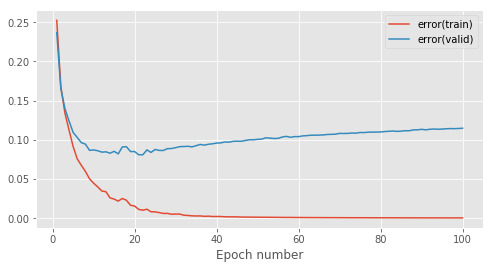
\includegraphics[width=\columnwidth]{relu2e.png}}
\caption{Error of ReLU. The minimum of validation error is 8.09e-02}
\label{fig:sample-graph}
\end{center}
\vskip -5mm
\end{figure}
\begin{figure}[htb]
\vskip 5mm
\begin{center}
\centerline{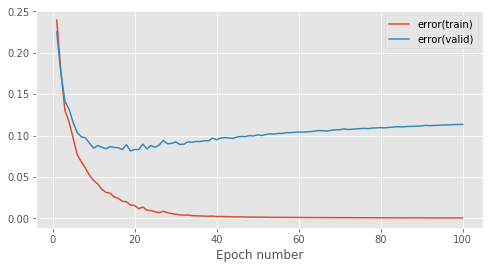
\includegraphics[width=\columnwidth]{lrelu2e.png}}
\caption{Error of Leaky ReLU. The minimum of validation error is 8.13e-02}
\label{fig:sample-graph}
\end{center}
\vskip -5mm
\end{figure}
\begin{figure}[tb]
\vskip 5mm
\begin{center}
\centerline{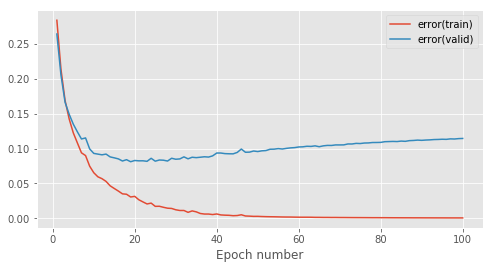
\includegraphics[width=\columnwidth]{elu2e.png}}
\caption{Error of ELU. The minimum of validation error is 8.12e-02}
\label{fig:sample-graph}
\end{center}
\vskip -5mm
\end{figure}
\begin{figure}[tb]
\vskip 5mm
\begin{center}
\centerline{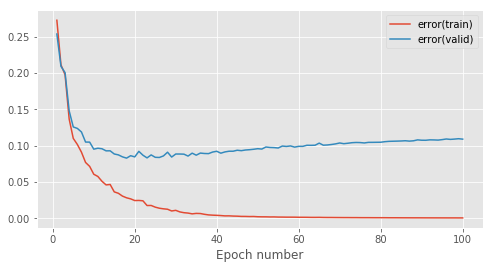
\includegraphics[width=\columnwidth]{selu2e.png}}
\caption{Error of SELU. The minimum of validation error is 8.29e-02}
\label{fig:sample-graph}
\end{center}
\vskip -5mm
\end{figure}
\begin{figure}[tb]
\vskip 5mm
\begin{center}
\centerline{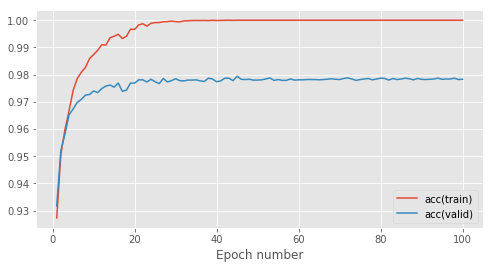
\includegraphics[width=\columnwidth]{relu2a.png}}
\caption{Accuracy of ReLU, the last accuracy of validation set is 9.78e-01}
\label{fig:sample-graph}
\end{center}
\vskip -5mm
\end{figure}
\begin{figure}[tb]
\vskip 5mm
\begin{center}
\centerline{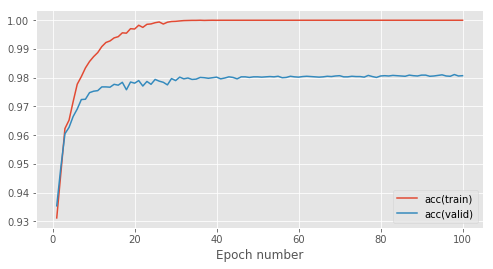
\includegraphics[width=\columnwidth]{lrelu2a.png}}
\caption{Accuracy of Leaky ReLU, the last accuracy of validation set is 9.81e-01}
\label{fig:sample-graph}
\end{center}
\vskip -5mm
\end{figure}
\begin{figure}[tb]
\vskip 5mm
\begin{center}
\centerline{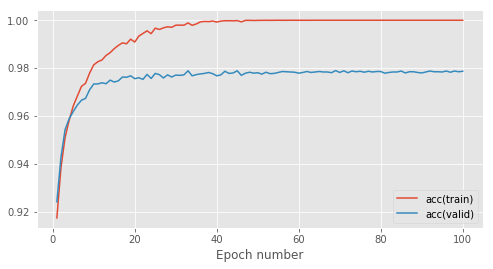
\includegraphics[width=\columnwidth]{elu2a.png}}
\caption{Accuracy of ELU, the last accuracy of validation set is 9.79e-01}
\label{fig:sample-graph}
\end{center}
\vskip -5mm
\end{figure}
\begin{figure}[tb]
\vskip 5mm
\begin{center}
\centerline{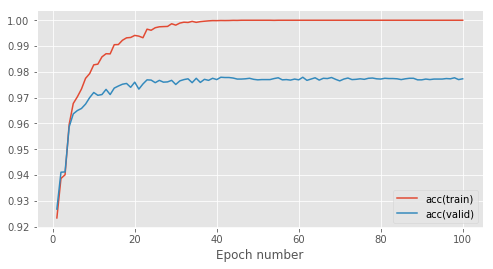
\includegraphics[width=\columnwidth]{selu2a.png}}
\caption{Accuracy of SELU, the last accuracy of validation set is 9.77e-01}
\label{fig:sample-graph}
\end{center}
\vskip -5mm
\end{figure}
% \begin{figure}[htbp]
%   \begin{minipage}{0.5\hsize}
%     \begin{center}
%       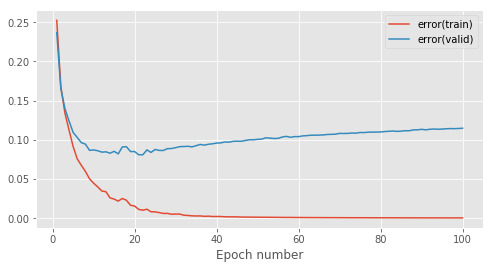
\includegraphics[width=70mm]{relu2e.png}
%     \caption{Error of ReLU}
%     \end{center}
%     \label{fig:img1}
%   \end{minipage}
%   \begin{minipage}{0.5\hsize}
%     \begin{center}
%       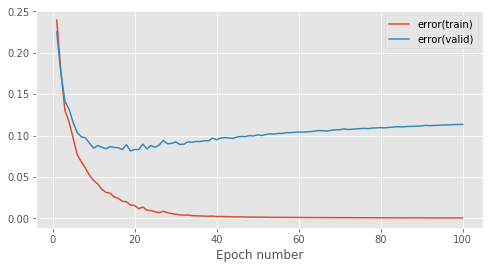
\includegraphics[width=70mm]{lrelu2e.png}
%     \caption{Error of Leaky ReLU}
%   \end{center}
%     \label{fig:img2}
%   \end{minipage}
%   \begin{minipage}{0.5\hsize}
%     \begin{center}
%       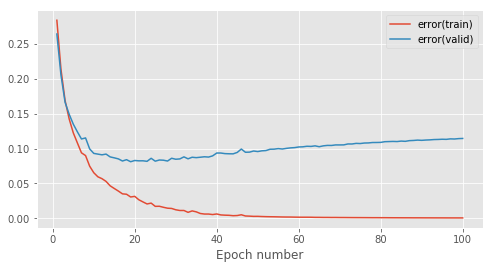
\includegraphics[width=70mm]{elu2e.png}
%     \end{center}
%     \caption{Error of ELU}
%     \label{fig:img3}
%   \end{minipage}
%   \begin{minipage}{0.5\hsize}
%     \begin{center}
%       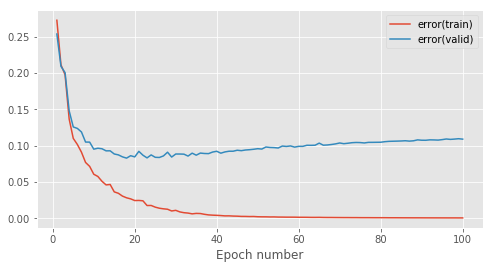
\includegraphics[width=70mm]{selu2e.png}
%     \end{center}
%     \caption{Error of SELU}
%     \label{fig:img4}
%   \end{minipage}
% \end{figure}

Next, look at the accuracy (Figure5-7).Only network with Leaky Relu function marks more than 0.98 validation accuracy.
Based on these result,contrary to expectations, Leaky Relu function achive the best perfomance on MNIST data although this function is older than ELU and SELU.

When the network has more layers, there might be more differences between models. However, this case there is only two hidden layers, so there are slight differences.

% Your experimental sections should include graphs (for instance, figure~\ref{fig:sample-graph}) and/or tables (for instance, table~\ref{tab:sample-table})\footnote{These examples were taken from the ICML template paper.}, using the \verb+figure+ and \verb+table+ environments, in which you use \verb+\includegraphics+ to include an image (pdf, png, or jpg formats).  Please export graphs as
% \href{https://en.wikipedia.org/wiki/Vector_graphics}{vector graphics}
% rather than \href{https://en.wikipedia.org/wiki/Raster_graphics}{raster
% files} as this will make sure all detail in the plot is visible.
% Matplotlib supports saving high quality figures in a wide range of
% common image formats using the
% \href{http://matplotlib.org/api/pyplot_api.html\#matplotlib.pyplot.savefig}{\texttt{savefig}}
% function. \textbf{You should use \texttt{savefig} rather than copying
% the screen-resolution raster images outputted in the notebook.} An
% example of using \texttt{savefig} to save a figure as a PDF file (which
% can be included as graphics in a \LaTeX document is given in the coursework document.
%
% If you need a figure or table to stretch across two columns use the \verb+figure*+ or \verb+table*+ environment instead of the \verb+figure+ or \verb+table+ environment.  Use the \verb+subfigure+ environment if you want to include multiple graphics in a single figure.
%
% \begin{figure}[tb]
% \vskip 5mm
% \begin{center}
% \centerline{\includegraphics[width=\columnwidth]{icml_numpapers}}
% \caption{Historical locations and number of accepted papers for International
%   Machine Learning Conferences (ICML 1993 -- ICML 2008) and
%   International Workshops on Machine Learning (ML 1988 -- ML
%   1992). At the time this figure was produced, the number of
%   accepted papers for ICML 2008 was unknown and instead estimated.}
% \label{fig:sample-graph}
% \end{center}
% \vskip -5mm
% \end{figure}
%
% \begin{table}[tb]
% \vskip 3mm
% \begin{center}
% \begin{small}
% \begin{sc}
% \begin{tabular}{lcccr}
% \hline
% \abovespace\belowspace
% Data set & Naive & Flexible & Better? \\
% \hline
% \abovespace
% Breast    & 95.9$\pm$ 0.2& 96.7$\pm$ 0.2& $\surd$ \\
% Cleveland & 83.3$\pm$ 0.6& 80.0$\pm$ 0.6& $\times$\\
% Glass2    & 61.9$\pm$ 1.4& 83.8$\pm$ 0.7& $\surd$ \\
% Credit    & 74.8$\pm$ 0.5& 78.3$\pm$ 0.6&         \\
% Horse     & 73.3$\pm$ 0.9& 69.7$\pm$ 1.0& $\times$\\
% Meta      & 67.1$\pm$ 0.6& 76.5$\pm$ 0.5& $\surd$ \\
% Pima      & 75.1$\pm$ 0.6& 73.9$\pm$ 0.5&         \\
% \belowspace
% Vehicle   & 44.9$\pm$ 0.6& 61.5$\pm$ 0.4& $\surd$ \\
% \hline
% \end{tabular}
% \end{sc}
% \end{small}
% \caption{Classification accuracies for naive Bayes and flexible
% Bayes on various data sets.}
% \label{tab:sample-table}
% \end{center}
% \vskip -3mm
% \end{table}

\section{Deep neural network experiments}
\label{sec:dnnexpts}
This section shows the experiments on deeper networks for MNIST.  The two sets of experiments are to explore the impact of the depth of the network (number of hidden layers), and a comparison of different approaches to weight initialisation.

First, using Leaky ReLU Layer, the author test different networks with 2 - 8 hidden layers. The result is on Table 1.
The author expects that deeper network is easier to overfit, and the accuracy decreases. However, the accuracy does not change dynamically, and the validation error increases in proportion to the depth of network.
The accuracy is high enough, so the author expects that the accuracy does not improve anymore. Also, error increase because of overfitting, so it grows when there are more hidden layers.

\begin{table}[tb]
\vskip 3mm
\begin{center}
\begin{small}
\begin{sc}
\begin{tabular}{lcccr}
\hline
\abovespace\belowspace
Depth & Min of Valid Error & Last Valid Error & Valid Accuracy \\
\hline
\abovespace
2    & 8.16e-02 & 1.12e-01 & 9.79e-01\\
3    & 8.30e-02 & 1.33e-01 & 9.80e-01\\
4    & 9.11e-02 & 1.48e-01 &  9.78e-01\\
5    & 9.45e-02 & 1.48e-01 & 9.80e-01\\
6    & 9.27e-02 & 1.66e-01 & 9.78e-01\\
7    & 9.38e-02 & 1.74e-01 & 9.80e-01\\
8    & 8.88e-02 & 1.74e-01 & 9.80e-01\\

\hline
\end{tabular}
\end{sc}
\end{small}
\caption{Relationship between depth of network and performance}
\label{tab:sample-table}
\end{center}
\vskip -3mm
\end{table}

Next, the author compares two initialization method, Glorot and Bengio's combined initialization, and Fan-in, Fan-out.
These initialization function is this:
\begin{equation}
  \begin{split}
  Fan-in: w_i \textasciitilde U(-\sqrt{3/n_{in}}, \sqrt{3/n_{in}}) \\
  Fan-out: w_i \textasciitilde U(-\sqrt{3/n_{out}}, \sqrt{3/n_{out}}) \\
  Glorot and Bengio's: w_i \textasciitilde U(-\sqrt{6/(n_{in}+n_{out})}, \sqrt{6/(n_{in}+n_{out})}) \\
  \end{split}
\end{equation}
where U is the uniform distribution.$n_{in}$ is the number of incoming connections, and $n_{out}$ is the number of outcoming connections.

This experiments uese layers with tow hidden LReLU layers and eight hidden LReLU layers.The result is on Table 2.

\begin{table*}[htb]
\vskip 3mm
\begin{center}
\begin{small}
\begin{sc}
\small
\begin{tabular}{lcccr}
\hline
\abovespace\belowspace
Depth & Initializer & Min of Valid Error & Last Valid Error & Valid Accuracy \\
\hline
\abovespace
2 &  GB & 8.16e-02 & 1.12e-01 & 9.79e-01\\
8 &  GB & 8.88e-02 & 1.74e-01 & 9.80e-01\\
2 &  Fan-in & 8.88e-02 & 1.19e-01 & 9.77e-01\\
8 &  Fan-in & 9.51e-02 & 1.84e-01 & 9.79e-01\\
2 &  Fan-out & 7.61e-02 & 1.04e-01 & 9.81e-01\\
8 &  Fan-out & 9.52e-02 & 1.65e-01 & 9.79e-01\\
\hline
\end{tabular}
\end{sc}
\end{small}
\caption{Relationship between initialisation and performance}
\label{tab:sample-table}
\end{center}
\vskip -3mm
\end{table*}

It show that the nework with 2 hidden layers and Fan-out initialiser mark the best performance. However, the graph of Glorot and Bengio's combined initialization is smoother (Figure 2, 10), so the Glorot and Bengio's approach makes learning stable.


\begin{figure}[tb]
\vskip 5mm
\begin{center}
\centerline{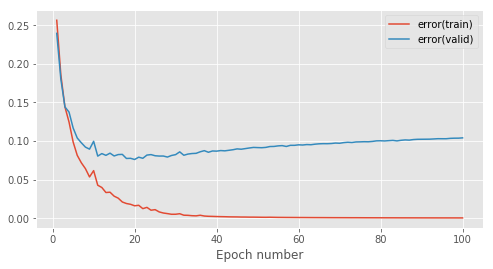
\includegraphics[width=\columnwidth]{faninn2e.png}}
\caption{Accuracy or of 2 layers, Leaky Relu, Fan-out initialization}
\label{fig:sample-graph}
\end{center}
\vskip -5mm
\end{figure}
\begin{figure}[tb]
\vskip 5mm
\begin{center}
\centerline{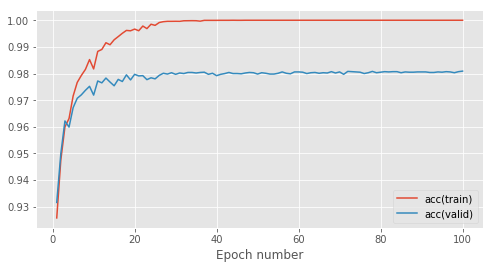
\includegraphics[width=\columnwidth]{faninn2aa.png}}
\caption{Error of 2 layers, Leaky Relu, Fan-out initialization}
\label{fig:sample-graph}
\end{center}
\vskip -5mm
\end{figure}

Also, the author test initialiation for SELU layer recommended by Klambauer et al. [2017]. This function is based on Gaussian distribution with mean 0 and variance $1/n_{in}$ .

The result is on Table 3.

It shows that the reccomendation strategy does not wrok better than Glorot and Bengio's combined initialization.

\begin{table*}[htb]
\vskip 3mm
\begin{center}
\begin{small}
\begin{sc}
\small
\begin{tabular}{lcccr}
\hline
\abovespace\belowspace
Depth & Initializer & Min of Valid Error & Last Valid Error & Valid Accuracy \\
\hline
\abovespace
2 &  GB & 8.38e-02 & 1.09e-01 & 9.77e-01\\
2 &  Gaussian & 9.36e-02 & 1.25e-01 & 9.76e-01\\
\hline
\end{tabular}
\end{sc}
\end{small}
\caption{Relationship between initialisation and performance with SELU layer}
\label{tab:sample-table}
\end{center}
\vskip -3mm
\end{table*}

% In this section, and in the previous section, you should present your experimental results clearly and concisely, followed by an interpretation and discussion of results. You need to present your results in a way that makes it easy for a reader to understand what they mean. You should facilitate comparisons either using graphs with multiple curves or (if appropriate, e.g. for accuracies) a results table. You need to avoid having too many figures, poorly labelled graphs, and graphs which should be comparable but which use different axis scales. A good presentation will enable the reader to compare trends in the same graph -- each graph should summarise the results relating to a particular research (sub)question.

% Your discussion should interpret the results, both in terms of summarising the outcomes of a particular experiment, and attempting to relate to the underlying models. A good report would have some analysis, resulting in an understanding of why particular results are observed, perhaps with reference to the literature. Use bibtex to organise your references -- in this case the references are in the file \verb+example-refs.bib+.  Here is a an example reference \citep{langley00}.



\section{Conclusions}
\label{sec:concl}
% You should draw conclusions from the experiments, related to the research questions outlined in the introduction (section~\ref{sec:intro}). You should state the conclusions clearly and concisely. It is good if the conclusion from one experiment influenced what you did in later experiments -- your aim is to learn from your experiments. Extra credit if you relate your findings to what has been reported in the literature.
%
% A good conclusions section would also include a further work discussion, building on work done so far, and referencing the literature where appropriate.

In these experiments, the network with Fan-out initialization, two layers, Leaky ReLU layer marks the best performance. However, this result is against the recent study. This time, the data set is simple, and networks are extremely deep. The SELU functions and initialization come into their own when predicting more complex data with deeper network.
% \bibliography{example-refs}

\end{document}


% This document was modified from the file originally made available by
% Pat Langley and Andrea Danyluk for ICML-2K. This version was
% created by Lise Getoor and Tobias Scheffer, it was slightly modified
% from the 2010 version by Thorsten Joachims & Johannes Fuernkranz,
% slightly modified from the 2009 version by Kiri Wagstaff and
% Sam Roweis's 2008 version, which is slightly modified from
% Prasad Tadepalli's 2007 version which is a lightly
% changed version of the previous year's version by Andrew Moore,
% which was in turn edited from those of Kristian Kersting and
% Codrina Lauth. Alex Smola contributed to the algorithmic style files.
 &
